\chapter{Methodology}
\label{ch:methodology}

This thesis employs the Design Science Research Methodology (DSRM) as introduced by \citet{peffersDesignScienceResearch2007} to structure the research process.
Design science research differs fundamentally from theory-building research.
Whereas natural and social sciences seek to understand and explain reality, design science creates and evaluates artifacts that solve identified organizational problems.
These artifacts can be constructs, models, methods, or instantiations \citep{peffersDesignScienceResearch2007}.

DSRM provides a six-activity process model \citep{peffersDesignScienceResearch2007}:
\begin{enumerate}
	\item problem identification and motivation,
	\item objectives of a solution,
	\item design and development,
	\item demonstration,
	\item evaluation, and
	\item communication.
\end{enumerate}
While presented sequentially, researchers may enter at different points.
The entry point depends on whether the research originates from an observed problem, desired objectives, an existing artifact, or a client need.
This flexibility accommodates the iterative nature of design work.
Evaluation findings inform refinements to the artifact throughout the research process \citep{peffersDesignScienceResearch2007}.

DSRM is particularly appropriate for this thesis.
The research creates and evaluates a designed artifact---a containerized development environment system.
This artifact addresses the identified problem of reproducibility and consistency in legacy software development.
The methodology ensures both rigor through systematic evaluation and relevance through solving practical organizational problems.

This research follows a \textit{problem-centered initiation}.
It begins with observed challenges in enterprise legacy software development.
The research then proceeds through solution design, implementation, and evaluation.

Figure \ref{fig:DSRM_Process_Model} illustrates the DSRM process model.
The following sections describe how each phase was applied to integrate containerization into legacy software development workflows.

\begin{figure}[htbp]
	\centering
	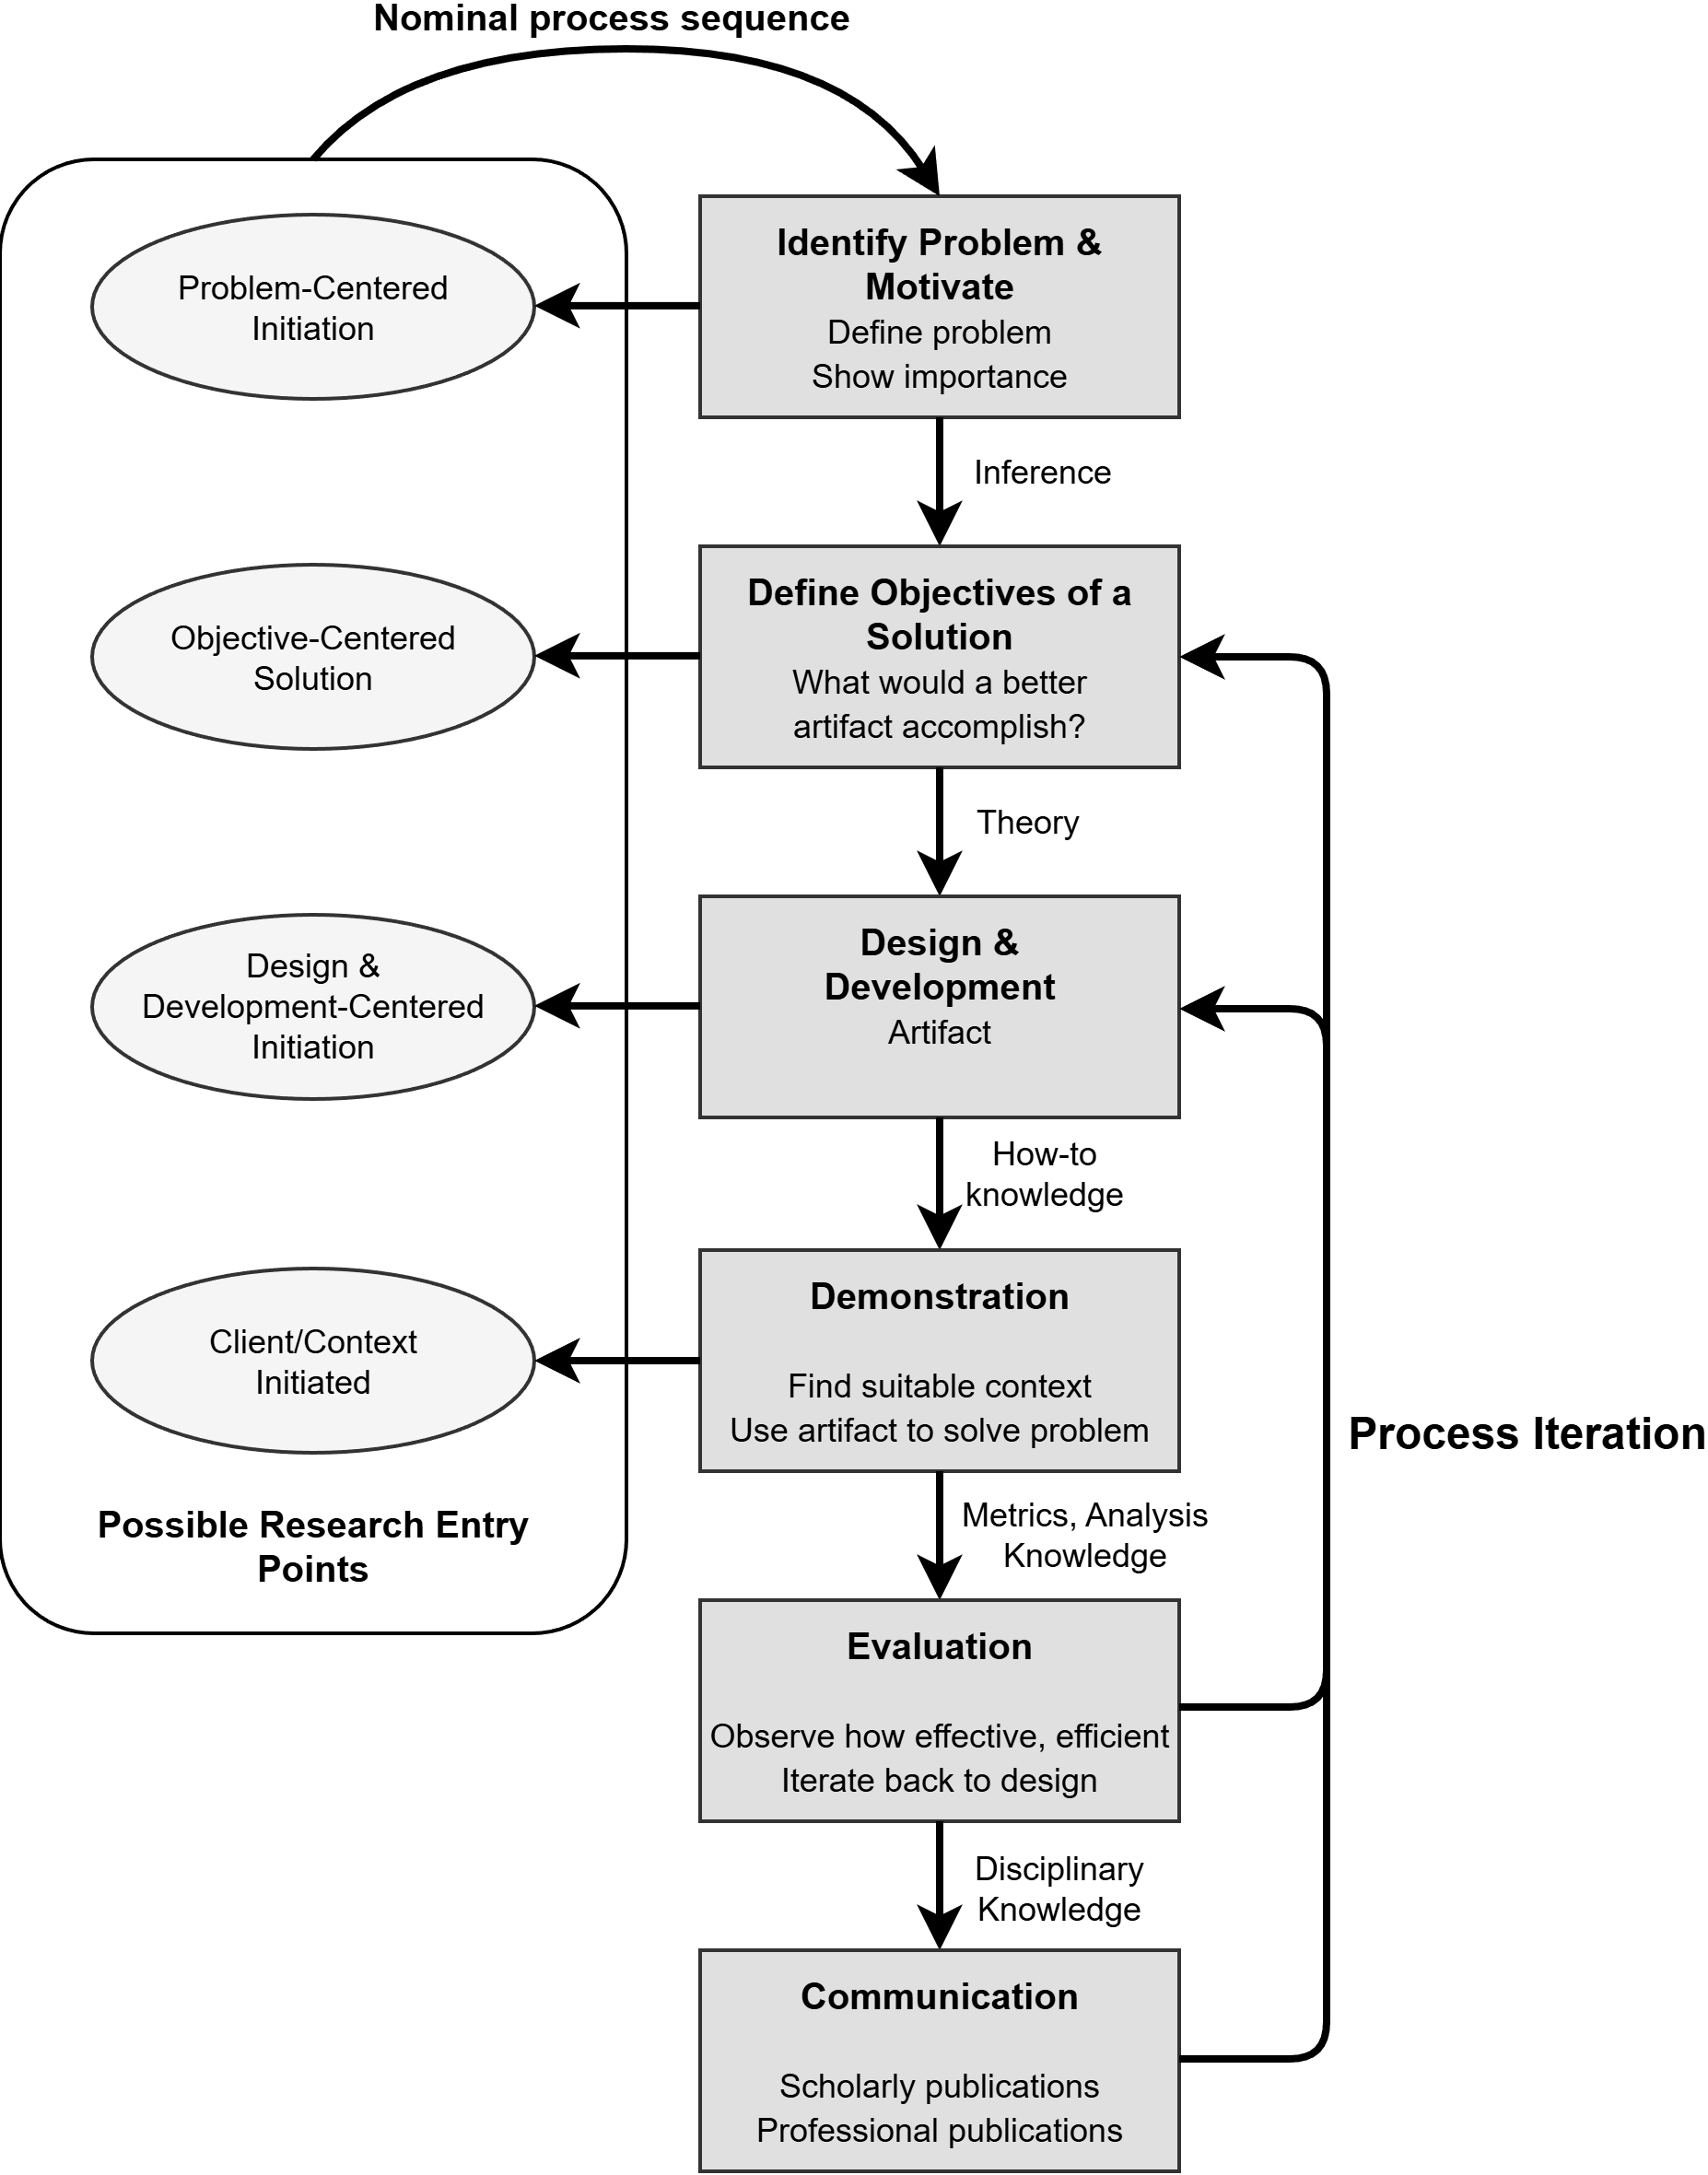
\includegraphics[width=0.98\linewidth]{figures/DSRM_Process_Model.png}
	\caption{DSRM Process Model (adapted from \cite{peffersDesignScienceResearch2007})}
	\label{fig:DSRM_Process_Model}
\end{figure}

\newpage
\section{Problem Identification and Motivation}

The first phase of DSRM involves defining the specific research problem and justifying the value of a solution \citep{peffersDesignScienceResearch2007}.
This phase establishes the foundation for subsequent design activities by articulating what problem the artifact should address.

Legacy software development projects, such as the WinCC Open Architecture system with its 30-year codebase, face significant challenges in maintaining reproducible and consistent development environments.
Manual setup processes introduce configuration drift, where development environments gradually diverge from intended configurations over time \citep{humbleContinuousDeliveryReliable2011}.
Developers working on Windows must validate their changes against Linux builds, historically relying on server-based builds for cross-platform verification.
This introduces delays in the development feedback loop and reduces developer productivity.

The problem-centered initiation of this research emerges from practical challenges observed in enterprise software development: reproducibility in legacy software development projects is difficult to achieve with traditional approaches.
The research question formulated in Chapter \ref{ch:introduction} captures this problem directly: \textit{How can containers be integrated in software development tasks for legacy software development projects?}
The sub-questions further specify the need to understand performance implications regarding build times (RQ1.1) and resource utilization (RQ1.2).

\section{Objectives of a Solution}

The second phase involves inferring the objectives of a solution from the problem definition \citep{peffersDesignScienceResearch2007}.
These objectives provide quantitative or qualitative criteria against which the artifact can be evaluated.

Based on the identified problems, four primary objectives guide the solution design:

\begin{enumerate}
	\item \textbf{Automated Environment Provisioning:} The solution should enable automated, reproducible development environment provisioning across heterogeneous platforms, eliminating manual configuration steps that introduce variability and human error.
	\item \textbf{Cross-Platform Build System Standardization:} The solution should provide unified build configurations that produce consistent results regardless of the underlying host operating system, addressing the common ``works on my machine'' problem.
	\item \textbf{Developer Experience Optimization:} The solution should integrate seamlessly with existing IDE workflows, enabling developers to leverage containerization benefits without requiring deep expertise in container technologies.
	\item \textbf{Performance Measurement Capabilities:} The solution should enable systematic comparison of build times, CPU utilization, and memory consumption across native, virtualized, and containerized environments to answer research questions RQ1.1 and RQ1.2.
\end{enumerate}

These objectives directly map to the functional requirements specified in Chapter \ref{ch:prototype_architecture}, ensuring alignment between research methodology and prototype design.

\section{Design and Development}

The third phase involves creating the artifact, which can be constructs, models, methods, or instantiations \citep{peffersDesignScienceResearch2007}.
This phase draws on existing theoretical foundations and applies them to create a solution that addresses the defined objectives.

The artifact developed for this thesis is a prototype development environment system comprising:

\begin{itemize}
	\item \textbf{Docker containers} for Linux development environments, utilizing multi-stage builds and DevContainer specifications for IDE integration
	\item \textbf{Hyper-V virtual machines} for cross-platform evaluation on Windows 11 hosts, enabling comparison between containerized and virtualized approaches
	\item \textbf{CMake preset configurations} for build system standardization across all environment types
	\item \textbf{A Python-based benchmark monitor} for capturing performance metrics during development operations
\end{itemize}

The prototype architecture is documented using the 4+1 Architectural View Model \citep{kruchten4+1ViewModel1995}, which provides a comprehensive framework for describing software-intensive systems through multiple concurrent views.
Chapter \ref{ch:prototype_architecture} presents the detailed design across logical, development, process, physical, and scenario perspectives.

The design decisions reflect infrastructure-as-code principles \citep{humbleContinuousDeliveryReliable2011}, ensuring that development environments are version-controlled, reproducible, and maintainable alongside the application source code.

\section{Demonstration}

The fourth phase demonstrates the use of the artifact to solve the identified problem \citep{peffersDesignScienceResearch2007}.
This involves applying the artifact in a suitable context through experimentation, simulation, case study, or other appropriate demonstration methods.

The prototype is demonstrated through two evaluation scenarios defined in Chapter \ref{ch:prototype_architecture}:

\textbf{Scenario 1: Toolchain Switching} measures the time required to switch between different development toolchains across native, containerized, and virtualized approaches.
This scenario addresses the practical challenge of developers needing to work with multiple compiler versions or validate cross-distribution compatibility.
The scenario compares:
\begin{itemize}
	\item Native Windows: Visual Studio reinstallation for version switching
	\item Containerized: Container image switching between different environments
	\item Virtualized: Hyper-V VM template switching between pre-configured environments on Windows 11 hosts
\end{itemize}

\newpage
\textbf{Scenario 2: Comprehensive Performance Benchmarking} measures build, installation, and test execution performance across all environment types with infrastructure already provisioned.
This scenario captures:
\begin{itemize}
	\item Clean build performance with cleared compiler caches
	\item CMake configuration timing
	\item Installation workflow timing
	\item Test execution performance
	\item Incremental feature addition overhead
	\item Compiler cache impact using sccache
	\item Resource utilization (CPU and memory) during all operations
\end{itemize}

The demonstration occurs on common workstations with controlled configurations to ensure reproducible measurements.
Windows 11 hosts with Hyper-V (for virtualization testing), Docker Desktop with WSL2 (for containerization with dynamic memory allocation to maximum 20GB RAM and 20 logical cores), and native development toolchains are evaluated.
Linux Debian 12 hosts with Docker Engine (unrestricted resources) and native development toolchains are also evaluated.
All virtual machines are allocated all logical cores (20 vCPUs) and 20GB memory (dynamic allocation to maximum 20GB for Windows guests; static 20GB allocation for Debian guests) to ensure comparable CPU utilization to native machines and eliminate artificial resource constraints.

\section{Evaluation}
\label{sec:methodology_evaluation}

The fifth phase observes and measures how well the artifact supports a solution to the problem \citep{peffersDesignScienceResearch2007}.
This involves comparing the objectives of a solution to actual observed results from use of the artifact.

The evaluation framework addresses the research questions through both architectural analysis and quantitative measurement.
Research question RQ1 is evaluated qualitatively by demonstrating how the prototype architecture achieves container integration through standardized build systems, IDE workflow preservation, and automated environment provisioning.
Sub-questions RQ1.1 and RQ1.2 are evaluated quantitatively through performance measurements across environment types.

The quantitative evaluation employs the following metrics:

\textbf{Build Time Metrics (RQ1.1):}
\begin{itemize}
	\item Clean build duration across native, VM, and container environments
	\item CMake configuration time
	\item Incremental build time for feature additions
	\item Compiler cache effectiveness
\end{itemize}

\newpage
\textbf{Resource Utilization Metrics (RQ1.2):}
\begin{itemize}
	\item System CPU and memory utilization during build operations
	\item Baseline measurements to isolate operation overhead from background activity
	\item Host system memory consumption when running Windows guests in VMs and when running containers via Docker Desktop on Windows hosts
\end{itemize}

\textbf{Environment Setup Metrics:}
\begin{itemize}
	\item Toolchain switching time (teardown and setup phases)
	\item Initial environment provisioning time for new developers
\end{itemize}

The benchmark monitor captures metrics at regular intervals during operations, logging results to structured JSON files for statistical analysis.
Each configuration is tested and measured with 30 repetitions.
To validate whether observed performance differences between environment types are statistically significant, two-tailed independent samples t-tests are applied to compare pairwise configurations \citep{montgomeryDesignAnalysisExperiments2017}.
The null hypothesis assumes no significant difference in mean performance between compared environments, with statistical significance evaluated at the conventional $\alpha = 0.05$ level.
Two-tailed tests are employed to detect performance differences in either direction without assuming a priori which environment will perform better.

The evaluation compares observed performance across environment types, quantifying the overhead or advantage of containerized development relative to native and virtualized baselines.
Results are presented in Chapter \ref{ch:empirical_results_evaluation} and discussed in Chapter \ref{ch:discussion}.

\section{Communication}

The sixth phase communicates the problem and its importance, the artifact, its utility and novelty, and the rigor of its design to relevant audiences \citep{peffersDesignScienceResearch2007}.

This thesis serves as the primary communication artifact, presenting:
\begin{itemize}
	\item The problem context of legacy software development challenges (Chapter \ref{ch:introduction})
	\item Theoretical foundations including containerization, virtualization, and development environment concepts (Chapter \ref{ch:fundamentals})
	\item Related work in development environment modernization (Chapter \ref{ch:related_work})
	\item The prototype design and architecture (Chapter \ref{ch:prototype_architecture})
	\item Empirical results from the evaluation scenarios (Chapter \ref{ch:empirical_results_evaluation})
	\item Discussion of findings and their implications (Chapter \ref{ch:discussion})
	\item Conclusions (Chapter \ref{ch:conclusion})
\end{itemize}

The findings contribute to the body of knowledge on containerization in software development, providing empirical evidence for practitioners considering containerized development environments for legacy software projects.

\section{Research Entry Point and Iterative Nature}

DSRM supports multiple entry points depending on the research context \citep{peffersDesignScienceResearch2007}.
This research follows a \textit{problem-centered initiation}, where the research began with observation of practical challenges in legacy software development with WinCC Open Architecture.
The need for reproducible, cross-platform development environments that reduce manual configuration overhead motivated the investigation of containerization as a potential solution.

While DSRM phases are presented sequentially, design science research rarely proceeds in strict linear fashion.
As introduced in Section~\ref{sec:research_methodology}, this research unfolds through two iterative phases:

\textbf{Iteration 1 (IT1): Prototype Development and Initial Evaluation.}
The first iteration focuses on designing and developing the initial version of the containerized development environment prototype.
This phase prioritizes the core infrastructure: Docker container configurations, virtual machine setups for comparison, and the benchmark monitoring system.
Initial demonstrations validate that the prototype can successfully build the legacy software project across native, containerized, and virtualized environments.
Preliminary evaluation identifies refinement opportunities and validates the measurement approach.

\textbf{Iteration 2 (IT2): Refinement and Comprehensive Evaluation.}
Based on insights from the initial iteration, the prototype is refined to address identified limitations.
This iteration executes the full evaluation scenarios: toolchain switching measurements and comprehensive performance benchmarking across all environment configurations.
The collected data enables quantitative comparison of build times (RQ1.1) and resource utilization (RQ1.2), providing empirical evidence to address the research questions.

\section{Summary}

This chapter described the application of Design Science Research Methodology to structure the research process for investigating containerization in legacy software development.
The six DSRM phases --- problem identification, objectives definition, design and development, demonstration, evaluation, and communication --- provide a structured framework for creating and evaluating the prototype artifact.

The problem-centered initiation reflects real-world challenges observed in enterprise software development, while the quantitative evaluation framework enables systematic comparison of development environment approaches.
The following chapters present the empirical results (Chapter \ref{ch:empirical_results_evaluation}) and discuss their implications for practitioners (Chapter \ref{ch:discussion}).
